\documentclass[12pt]{article}
\usepackage[utf8]{inputenc}
\usepackage{amsmath}
\usepackage{mathtools}
\usepackage{amsfonts}
\usepackage{lastpage}
\usepackage{tikz}
\usepackage{pdfpages}
\usepackage{gauss}
\usepackage{fancyvrb}
\usepackage{fancyhdr}
\usepackage{graphicx}
\pagestyle{fancy}
\fancyfoot[C]{\footnotesize Page \thepage\ of 6}
\DeclareGraphicsExtensions{.pdf,.png,.jpg}
\title{MatIntroNat}
\author{Nikolaj Dybdahl Rathcke}
\chead{Nikolaj Dybdahl Rathcke (rfq695)}

\begin{document}
\section*{MatIntroNat - Opgave 2}

\subsection*{Opgave 3.1}
Lad
$$f(x)=\frac{1}{x}-\frac{cosx}{sinx}$$
for alle $x\in \mathbb{R}$ med $x\neq n\pi,n\in \mathbb{Z}$

\subsubsection*{a}
Find grænseværdierne $lim_{x\rightarrow0^{+}} f(x)$, $lim_{x\rightarrow\pi^{-}} f(x)$ først med og dernæst uden Maple.\\
\\
Nedenfor ses grænseværdierne beregnet med Maple:\\
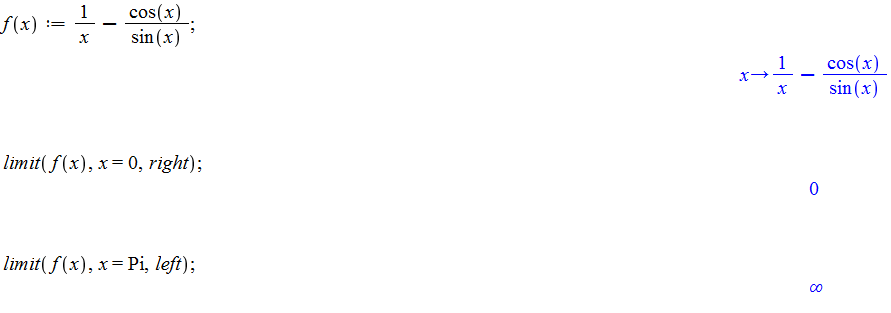
\includegraphics[scale=0.6]{Pic1}\\
Det ses, at $lim_{x\rightarrow0^{+}} f(x)=0$ og $lim_{x\rightarrow\pi^{-}} f(x)=\infty$.\\
\\
Nu beregnes det uden brug af Maple.\\
Vi starter med at omskrive $f(x)$ ved at gange højre led med $x$ i tæller og nævner og derefter gange venstre led med $sin(x)$ i tæller og nævner:
$$f(x)=\frac{sinx}{xsinx}-\frac{xcosx}{xsinx}=\frac{sinx-xcosx}{xsinx}$$
Hvis vi nu lader $x$ tilnærmse sig $0$ fra højre, får vi:\\
$$lim_{x\rightarrow0^{+}} f(x)=\frac{sinx-xcosx}{xsinx}$$
Da både tæller og nævner kommer til at gå mod 0 når $x$ går mod 0, kan vi bruge L'Hôspitals regel, som siger grænseværdien kan findes ved tæller differentieret over nævner differentieret. Vi får her det differentierede udtryk og kan reducere det ved hjælp af derivationsregler:
$$f'(x)=\frac{cosx-(cosx+x(-sinx))}{sinx+xcosx}=\frac{xsinx}{sinx+cosx}$$
Her ses, at tæller går mod $0$ når $x$ går mod $0$. Samtidig går nævner mod $1$ når $x$ går mod $0$, så vi har:
$$lim_{x\rightarrow0^{+}}\frac{xsinx}{sinx+cosx}=0$$
\\
Nu ønsker vi at finde $lim_{x\rightarrow\pi^{-}} f(x)$. Vi lader $x$ gå mod $\pi$ fra venstre.\\
$$lim_{x\rightarrow\pi^{-}} \frac{1}{\pi}-\frac{cos\pi}{sin\pi}$$
Her går $cosx$ mod $-1$ når $x$ går mod $\pi$ og $sinx$ går mod $0$ når $x$ går mod $\pi$. Vi får derfor at dette led går mod negativt uendelige:
$$lim_{x\rightarrow\pi^{-}} \frac{1}{\pi}-\frac{cos\pi}{sin\pi}=\frac{1}{\pi}-(-\infty)=\infty$$
Og grænseværdierne er fundet uden brug af Maple.

\subsubsection*{b}
Vis, at $f$ er strengt voksende i hvert interval $(n\pi,(n+1)\pi)$. Uligheden $|sinx|<|x|$ for $x\neq 0$ kan benyttes uden bevis.\\
\\
Hvis $f'(x)>0$ betyder det at $f$ er strengt voksende.\\
Vi kigger på den differentierede $f(x)$\\
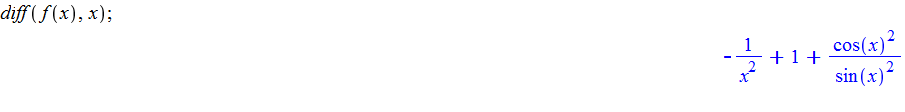
\includegraphics[scale=0.6]{Pic6}\\
Altså skal der gælde at
$$0<-\frac{1}{x^2}+1+\frac{cosx^2}{sinx^2}$$
Vi kan lave omskrivningerne:
$$0<-\frac{1}{x^2}+\frac{sinx^2}{sinx^2}+\frac{cosx^2}{sinx^2}$$
$$0<-\frac{1}{x^2}+\frac{cosx^2+sinx^2}{sinx^2}$$
Desuden kan vi bruge pythagoras på tælleren i det andet led på højre side og substituere $cosx^2+sinx^2=1$. Vi rykker desuden $\frac{1}{x^2}$ hen på den anden side af ulighedstegnet.
$$0<\frac{1}{sinx^2}-\frac{1}{x^2}$$
Ganger med $x^2$ i det første led på højre side og med $sinx^2$ i det andet led på højre side.
$$0<\frac{x^2-sinx^2}{sinx^2*x^2}$$
Da vi desuden kan bruge uligheden $|sinx|<|x|$ for $x\neq 0$ må det også gælde at $sinx^2<x^2$ og derved er tælleren positiv. Desuden må nævneren også være positiv da alle ledene der indgår er i anden potens. Altså er det vist at $f'(x) > 0$.

\subsubsection*{c}
Bevis, at ligningen $f(x)=0$ ikke har nogen løsninger i $(0,\pi)$ og at den har præcis en løsning i $(\pi,2\pi)$. Benyt Maple til at finde en approximation til denne løsning.\\
\\
Vi starter med at vise den ikke har nogen løsninger i $(0,\pi)$.\\
Vi allerede har kigget på grænseværdien for $x$ gående mod 0 fra højre, som var 0. Hvilket vil sige den aldrig vil blive præcist 0. Vi har også kigget på grænseværdien for $x$ gående mod $\pi$ fra venstre, som var uendelig. Da vi desuden i (b) viste at den er strengt voksende i alle intervaller $(n\pi,(n+1)\pi)$ kan vi ud fra skæringssætningen konkludere at den aldrig skærer x-aksen i netop dette interval.\\
\\
Nu ønsker vi at vise at den har en løsning i $(\pi,2\pi)$.\\
Vi starter med at kigge på grænseværdierne $lim_{x\rightarrow\pi^{+}}f(x)$ og $lim_{x\rightarrow2\pi^{-}}f(x)$:\\
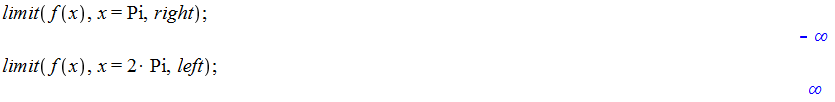
\includegraphics[scale=0.6]{Pic2}\\
Da vi kan se, at disse værdier ligger på hver side af $0$ og vi i (b) stadig har den er strengt voksende i alle intervaller $(n\pi,(n+1)\pi)$ kan vi bruge skæringssætningen til at sige der må være nøjagtigt en løsning $f(x)=0$ i dette interval. Denne approximerer vi med Maple:\\
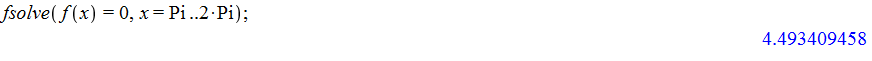
\includegraphics[scale=0.6]{Pic3}\\
Altså skærer $f(x)=0$ når $x\approx 4.49$.

\newpage

\subsection*{Opgave 3.2}
En funktion $f:\mathbb{R}\rightarrow\mathbb{R}$ defineres ved
$$f(x) = \left\{ \begin{array}{rl}
\frac{1-x^2}{(x-1)(x-3)} &\mbox{$x\in (-\infty;1)\cup(3;\infty)$} \\
x &\mbox{$x\in [1,3]$}
\end{array} \right.$$
\subsubsection*{a}
Lav i Maple et plot af et udsnit af grafen for $f$, der giver et retvisende og oplysende billede af funktionens overordnede opførsel.\\
\\
Nedenfor ses et plot af funktionen i Maple. Den er plottet omkring $x=1$ og $x=3$ da det er her funktionsudtrykket ændres:\\
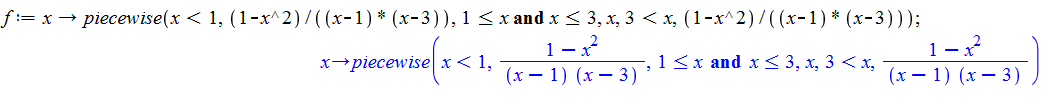
\includegraphics[scale=0.6]{Pic4}\\
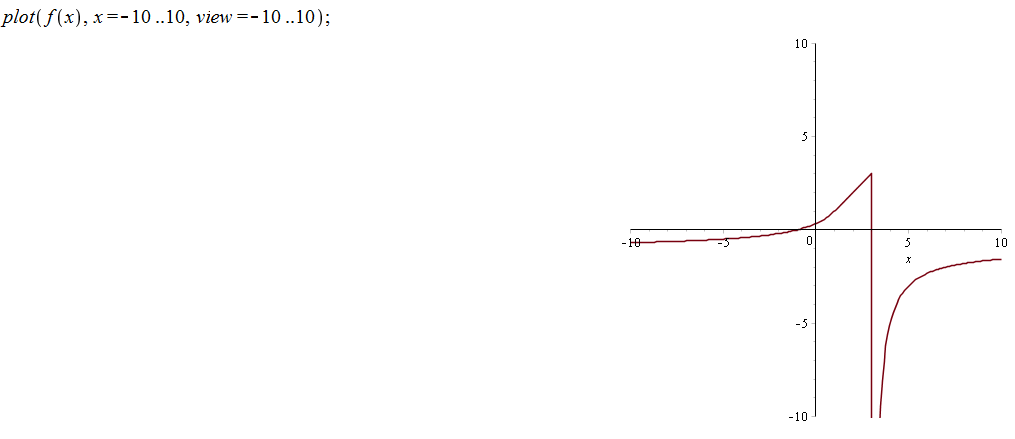
\includegraphics[scale=0.6]{Pic5}

\subsubsection*{b}
Er $f$ differentiabel i $x=1$? Begrund dit svar uden brug af Maple.\\
\\
Vi ønsker først at vise at funktionen er kontinuert i $x=1$. Dette gøres ved at kigge på grænseværdierne for begge funktionsudtryk.\\
$$lim_{x\rightarrow 1^{-}}f(x)\:og\:lim_{x\rightarrow 1^{+}}f(x)$$
Vi beregner $lim_{x\rightarrow 1^{-}}f(x)$
$$lim_{x\rightarrow 1^{-}}\frac{1-x^2}{(x-1)(x-3)}$$
Da indsættelse af $x=1$ giver et "$0/0$" udtryk benytter vi os af L'Hôpitals regel, som siger grænseværdien kan findes ved tæller differentieret over nævner differentieret.
$$lim_{x\rightarrow 1^{-}}\frac{1-x^2}{x^2-x-3x+3}=lim_{x\rightarrow 1^{-}}\frac{-2x}{2x-4}=1$$
Derefter beregnes $lim_{x\rightarrow 1^{+}}f(x)$
$$lim_{x\rightarrow 1^{+}}x=1$$
Altså er $f(x)$ kontinuert omkring $x=1$ da grænsen er den samme for begge funktionsudtryk.\\
Vi skal desuden vise
$$lim_{x\rightarrow 1^{\pm}}\frac{f(x)-f(a)}{x-a}$$
eksisterer entydigt.\\
Vi starter med at vise det for det første funktionsudtryk\\
$$lim_{x\rightarrow 1^{-}}\frac{\frac{1-x^2}{(x-1)(x-3)}-1}{x-1}$$
Igen benytter vi os a L'Hôpitals regel og får:
$$lim_{x\rightarrow 1^{-}}\frac{\frac{-2x}{2x-4}}{1}=lim_{x\rightarrow 1^{-}}\frac{-2x}{2x-4}=1$$
Vi får for det andet funktionsudtryk:
$$lim_{x\rightarrow 1^{+}}\frac{x-1}{x-1}=1$$
Og da disse begge går mod 1 er $f(x)$ altså differentiabel i $x=1$







\end{document}
